%!TEX root = ../thesis.tex

\newchap{Event simulation and reconstruction}\label{sec:RECO}
\vspace{-1cm}
\minitoc

\section{Event reconstruction}\label{sec:PF}
The event reconstruction is the identification of all the particles and their kinematics from each pp collision, starting from the raw data that is just a collection of hits and energy clusters.\\
CMS is a highly segmented detector, designed to give a different signature for each kind of particle.
All the charged particles produce tracks, electrons, and photons produce a shower in the ECAL, hadrons start showering in the ECAL and are absorbed in the HCAL, while muons, due to their mass, are minimum ionizing particles that penetrate all the detector, leaving tracks in the tracker and the muon system (\Fig{fig:PF}).
\begin{figure}[h!]
    \centering
    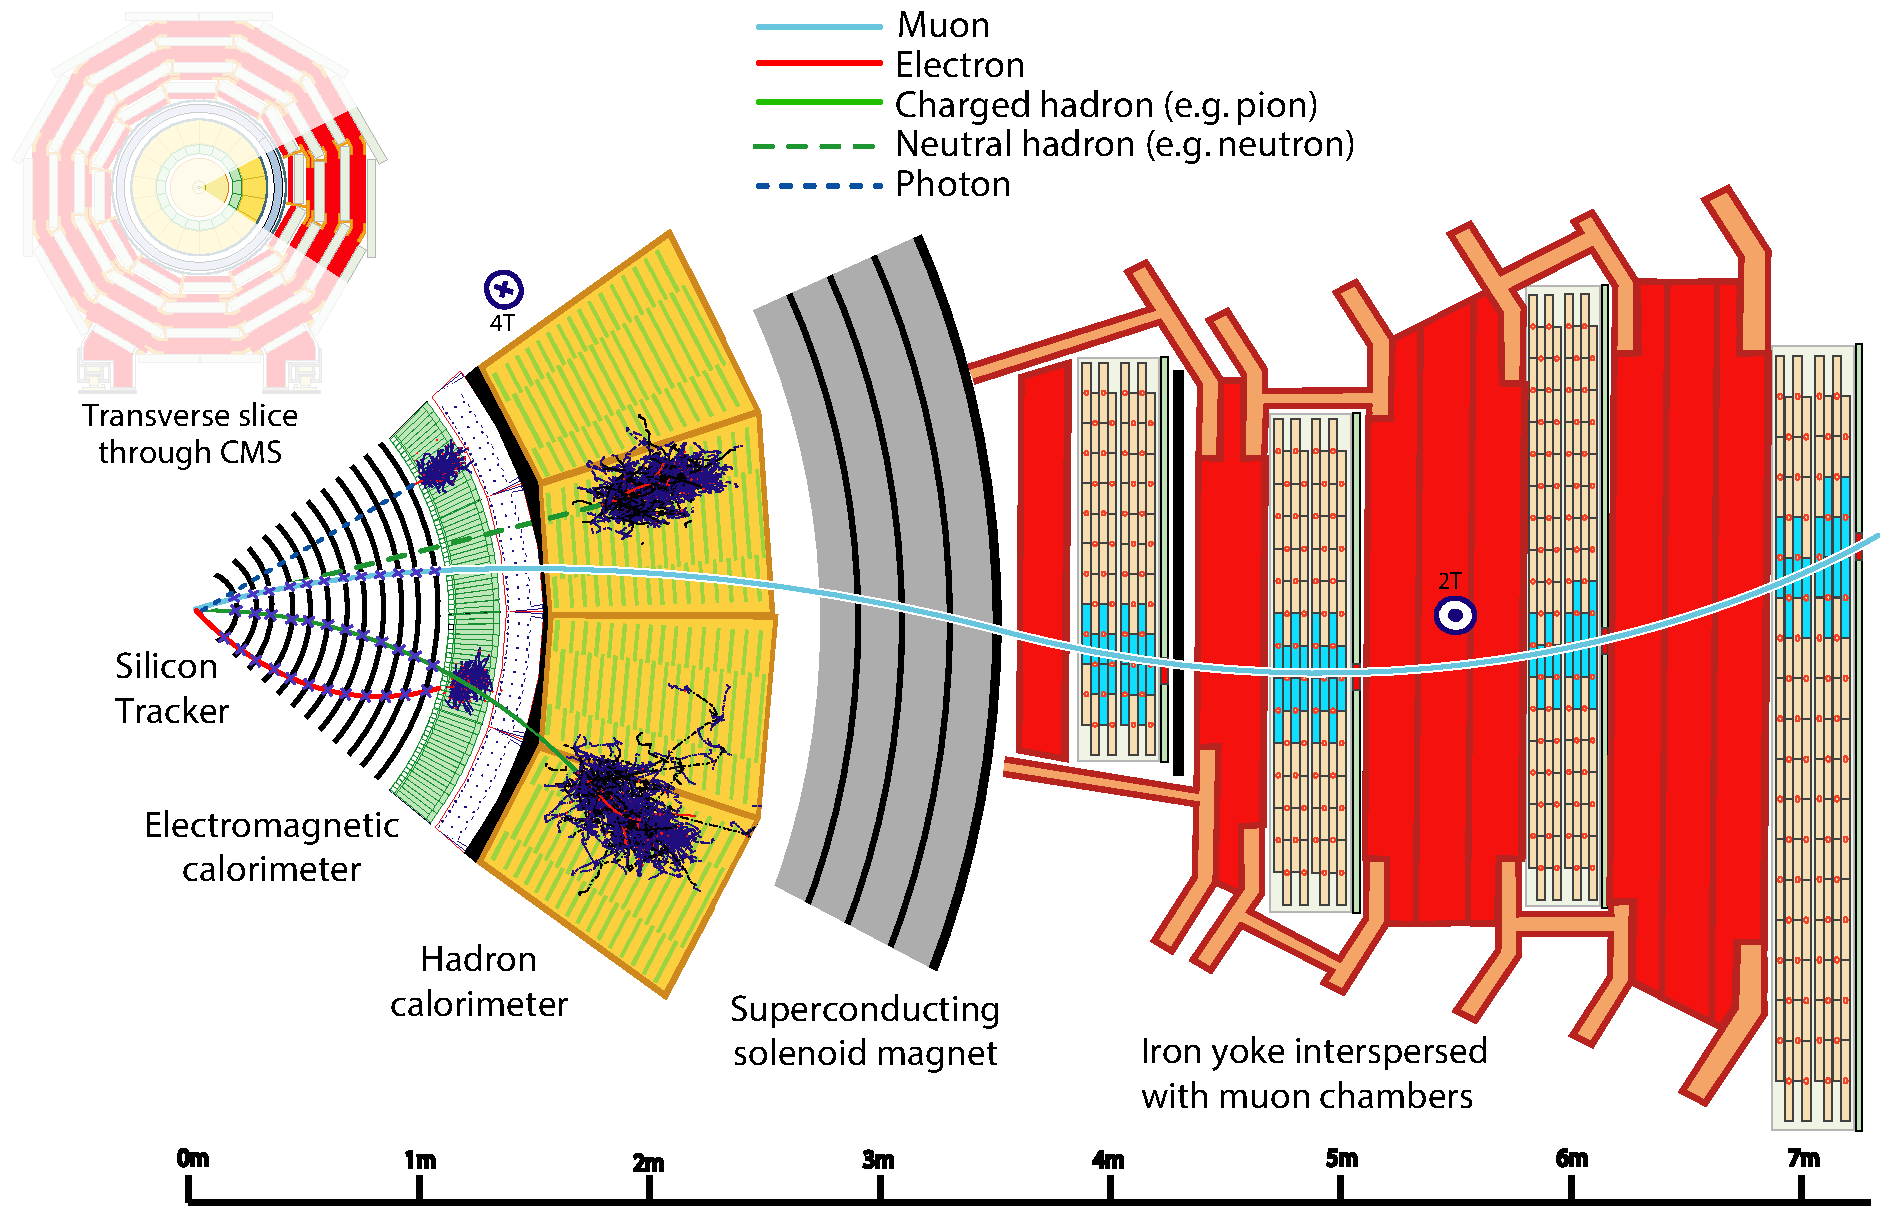
\includegraphics[width=\linewidth]{fig//chap04-reco/CMS_detector_PID_edit.pdf}
    \caption{Signatures of different types of particles in a slice of the CMS detector. The muon and the charged pion are positively charged, and the electron is negatively charged. \cite{Sirunyan2017Particle-flowDetector}}
    \label{fig:PF}
\end{figure}
\\
The informations of the different subdetectors are linked together to improve the resolution of the detector and to consider other signatures (\eg reconstructing a photon that has converted an electron-positron pair in the tracker).
This approach is called Particle Flow (PF) \cite{Sirunyan2017Particle-flowDetector}, and each reconstructed particle is called a PF candidate.



\subsection{Tracking}\label{sec:tracking}
The algorithm used to reconstruct the trajectories of charged particles and their momentum is the Combinatorial Track Finder (CTF) \cite{Chatrchyan2014DescriptionTracker}, an adaptation of the Kalman Filtering (KF) \cite{Fruhwirth1987ApplicationFitting} algorithm.
At the beginning, a few hits in consecutive layers of the tracker are used as seed of the KF algorithms and then a final fit is performed to estimate the position of the vertex, the direction, and the momentum of each charged particle.\\

\paragraph*{Seeding and iterations}
This process is iterated in multiple steps, starting with searching for tracks that are easier to find (\eg particle with large $p_T$ produced in the IP), removing the associated hits to reduce the combinatorial multiplicity, and searching for other kinds of tracks using different seeding criteria (Table \ref{tab:track_seeding}).

\begin{table}[h!]
    \centering
    \begin{tabular}{|c|c|c|c|}
    \hline
    Iteration&Name&Seeding&Targeted Tracks\\
    \hline
    1& InitialStep&pixel triplets&prompt, high $p_T$\\
    2& DetachedTriplet&pixel triplets&from b hadron decays, $R\leq 5$cm\\
    3& LowPtTriplet&pixel triplets&prompt, low $p_T$\\
    4& PixelPair&pixel pairs&recover high $p_T$\\
    5& MixedTriplet&pixel+strip&triplets displaced, $R\leq 7$cm\\
    6& PixelLess&strip triplets/pairs&very displaced, $R\leq 25$cm\\
    7& TobTec&strip triplets/pairs&very displaced, $R\leq 60$cm\\
    8& JetCoreRegional&pixel+strip pairs&inside high $p_T$ jets\\
    9& MuonSeededInOut&muon-tagged&tracks muons\\
    10& MuonSeededOutIn&muon detectors&muons \\
    \hline
    \end{tabular}
    \caption{Seeding configuration of ten iterations with different target tracks. $R$ is the target distance of the track origin from the beam axis \cite{Sirunyan2017Particle-flowDetector}. }
    \label{tab:track_seeding}
\end{table}

\paragraph*{Track finding}
The track finding is divided into four steps:
\begin{enumerate}
    \item Using the parameter of the track candidate (given by the seed at the beginning), determine which successive layer of the tracker can be intersected by the trajectory, considering its uncertainties.\\ The trajectories are assumed to be perfect Helix, neglecting the multiple scattering, allowing us to use fast analytical methods.
    \item Look for a compatible silicon module\footnote{Silicon modules usually overlap, so in this step the algorithms look for groups of modules, also to ease the computational effort.} in the layer such that its boundary is less than $3 \sigma$ from the trajectory. The trajectory and its uncertainties are propagated to the sensor surface.
    \item A $\chi^2$ test is used to check which of the hits are compatible with the track candidate, considering both the hit and the trajectory uncertainties.
    \item Update the track candidate and iterate
\end{enumerate}
\paragraph*{Track fitting}
To determine the track parameters, after all hits of each track are assigned by the track finder, a new KF fit is initialized at the location of the innermost hit. The fit proceeds through all the hits, from inside outwards.\\
This filter is followed by a smoothing stage that consists of a second KF initialized with the result of the first one and is run backward. The track parameters are obtained from a weighted average of the track parameters of these two filters.\\
During the track fitting stage, the effects of interaction with materials and  inhomogeneous of the magnetic field are considered.

\begin{figure}[H]
    \centering
    \includegraphics[width=0.75\linewidth]{fig//chap04-reco/KF.png}
    \caption{Visualization of the forward filter and the backward smoother filter. The red points indicate the measurements and their uncertainties on each layer, while the green points indicate the predictions \cite{Ai2021AFitting}.}
    \label{fig:KF}
\end{figure}

\subsubsection*{Muon tracks}
The reconstruction of muon tracks combines the information from the tracker and the muon system. Three types of tracks are defined:
\begin{itemize}
    \item \textbf{Standalone muons}: Tracks built using only the hits in the muon system.
    \item \textbf{Tracker muons}: Tracks built using only the hits in the tracker that match the track segments in the muon system.
    \item \textbf{Global muons}: Tracks fitted combining the tracker and the muon system hits, improving the $p_T$ resolution of the tracking detector.
\end{itemize}
Usually, there is no reason to not use global muons, but low $p_T$ muons can be reconstructed as tracker muons because of the large multiple scattering in the return yoke. 

\subsubsection*{Electron tracks}
The initial identification of electrons is performed in two ways:
The first consists of estimating the electron momentum from the $\phi$ spreading of the ECAL cluster and finding a track compatible with the cluster.
The second method consists of finding ECAL clusters compatible with tracks extrapolated  from the tracker.\\
\\
Electrons, traversing the tracker, radiate energy by Bremsstrahlung. For this reason, the KF doesn't perform well, so, tracks that are identified as electrons are refitted with the Gaussian sum filter (GSF) algorithm \cite{Adam2003ReconstructionLHC} that approximates the energy loss of electrons, described by the Bethe-Heitler distribution \cite{Bethe1934OnElectrons}, as a Gaussian mixture.\\
At each layer, a set of helical track segments is computed for a different value of the energy loss, and it's weighted with the corresponding probability of occurring. These informations are used to decrease the energy of the particle and update the trajectory uncertainties at each layer.
\subsubsection*{Vertex reconstruction}
Once all the tracks are reconstructed, those that come from the same vertex are clustered together and a fit is performed to determine the vertex position.\\
The fit is done using the simulated annealing algorithm \cite{Kirkpatrick1983OptimizationAnnealing} that estimates the vertex position by minimizing a free energy function and associates to each track the probability of belonging to the i-th vertex. \\

\subsection{Calorimeter clustering}
The clustering in calorimeters is necessary to reconstruct photons (in the ECAL) and neutral hadrons (in the HCAL), objects that don't leave any signature in the tracker system.\\
The ECAL is also used to improve the identification of electrons, matching the tracks with the ECAL energy clusters and looking for bremsstrahlung photons, and both the ECAL and the HCAL to improve the reconstruction of charged hadrons, especially the high energetic ones.\\
Cluster seeds are built from cells with an energy larger than a given threshold and
larger than the energy of the neighboring cells.\\
Starting from the seeds, topological clusters are built by aggregating neighboring cells that have an energy larger than twice the noise level.\\
Assuming that the energy deposit in the M cells contained in the topological cluster arises from N Gaussian energy deposits, one for each seed in the topological cluster, a Gaussian mixture model is used to reconstruct the cluster. The parameters of the Gaussian are the location parameters in the $(\eta,\phi)$ plane and the amplitude, while the width has a fixed value, different for each subdetector.\\
The energy and the position of the seeds are used as initial values for the parameters of the Gaussian mixture that are estimated through an analytical maximum likelihood fit.\\

\begin{table}[h!]
    \centering
    \begin{tabular}{|c|cc|cc|c|}
    \hline
    &\multicolumn{2}{c|}{ECAL} & \multicolumn{2}{c|}{HCAL} & Preshower\\
    &barrel&endcaps&barrel&endcaps& \\
    \hline
    Cell E threshold (MeV)&80&300&800&800&0.06\\
    Seed \# closest cells&8&8&4&4&8\\
    Seed E threshold (MeV)&230&600&800&1100&0.12\\
    Seed ET threshold (MeV)&0&150&0&0&0\\
    Gaussian width (cm)&1.5&1.5&10.0&10.0&0.2\\
    \hline
    \end{tabular}
    \caption{Seeding and clustering parameters for the ECAL, the HCAL, and the pre-showers \cite{Sirunyan2017Particle-flowDetector}.}
    \label{tab:clustering}
\end{table}

\subsection{ParticleFlow linking}
The PF elements are initially built separately in each subdetector and each of them can be linked with other PF elements in their k-nearest neighborhood \cite{Dasarathy1991NearestTechniques} (kNN) in the $(\eta,\phi)$ plane.\\
The linking algorithm assigns a distance between each possible pair of elements that quantifies the quality of the link. All elements that are linked together form a PF block.\\

\paragraph*{Track to track linking}
Charged particles that originate from a common secondary vertex and have an invariant mass greater than 0.2 \GeV are linked together to reconstruct a nuclear interaction or a displaced decay.

\paragraph*{Track-CaloCluster linking}
A track is linked to a calorimeter cluster if the position of the track in the $(\eta,\phi)$ plane ($(x,y)$ for the endcaps), extrapolated from the hit in the outermost layer, is contained in the union of the cluster areas of the ECAL and HCAL. The cluster areas are enlarged to take into account the uncertainties in the position, multiple scattering, and the presence of cracks between cells.\\
The link distance is defined as the distance between the track and the cluster in the $(\eta,\phi)$ plane for the barrel and in the $(x,y)$ plane for the endcaps, keeping only the link with the smallest distance for each element.\\
Furthermore, photons emitted tangent to electron tracks (with $|\Delta \eta| <0.5$) are collected as Bremsstrahlung photons. They have a significant probability of converting into electron-positron pairs, so a dedicated conversion finder algorithm \cite{Sirunyan2021ElectronLHC}, based on the iterative tracker procedure (discussed in sec \ref{sec:tracking}), is used to link $e^+e^-$ tracks to the corresponding photons.\\
In this step, the clusters associated with electrons and Bremsstrahlung photons are clustered into superclusters.



\paragraph*{Cluster to cluster linking}
When the cluster position of the more granular calorimeter is contained in the cluster area of the less granular calorimeter, the link is established.
Also in this case, the distance is defined as the distance of the cluster positions in the $(\eta,\phi)$ plane for the barrel and in the $(x,y)$ plane for the endcaps and just the link with the smallest distance is kept.

\paragraph*{Track-muon linking}
As explained in sec \ref{sec:tracking}, the PF elements in the tracker are linked with the ones in the muon system through spatial matching to allow the global fitting of the muon tracks.



\subsection{ParticleFlow reconstruction}
In each PF block, muon candidates are identified and reconstructed first. The following steps deal with the reconstruction of electrons, photons, and hadrons.
At each step, the PF blocks used to reconstruct the candidate are removed. In particular, the electron reconstruction is performed before the photon reconstruction to remove elements associated with Bremsstrahlung photons.\\
At the end, when all blocks have been processed, the event is revisited in a post-processing step.

\paragraph*{Muons}
To avoid the misidentification of hadrons in muons (that can occur for high-energy hadrons that reach the muon system), isolated global muons are selected by considering all the tracks and energy deposits within $\Delta R<0.3$ from the muon direction, with the constraint that: the scalar sum of the $p_T$ and the $E_T$ of other elements have to be less than the 10\% of the muon $p_t$; there are at least three track segments in the muon system; and the calorimeter deposit match the $p_t$ estimate from the track.\\
Muons originating from the semileptonic decay of hadrons require more stringent criteria.

\paragraph*{Electrons and photons}
Because electrons emit Bremsstrahlung photons and photons convert to electron pairs, the reconstruction of electrons and photons is performed in the same step.\\
For each supercluster, if it matches a GSF track, an electron candidate is built, if not, a photon candidate is built. \\
All the ECAL clusters in the PF block linked to the supercluster, to the electron track, or tracks belonging to a photon conversion are associated with the candidate.\\
Electron candidates must satisfy additional identification constraints on the amount of energy radiated, the distance between the track and the ECAL cluster in the $(\eta,\phi)$ plane, the ratio of the energy released in the ECAL and the HCAL, the number of hits and goodness of fit of the track reconstructed both with the KF and the GSF. The final identification of the electron is performed by a Boosted decision tree (BDT) that is trained on all these inputs.\\
Photons must satisfy isolation criteria that just require the isolation from other tracks and clusters.

\paragraph*{Hadrons}
The remaining PF blocks in the ECAL that are not linked with a track are identified as non-isolated photons originating from $\pi^0$ decays, while the ones in the HCAL as neutral hadrons.\\
The remaining HCAL clusters are linked to tracks and, eventually, to other remaining ECAL clusters to identify charged hadrons.\\
It is relevant to note that, outside the tracker coverage, charged and neutral hadrons cannot be distinguished anymore.

\paragraph*{Missing transverse momentum}
The neutrinos and other hypothetical exotic particles do not interact with the detector material and the only quantity that we can measure is the missing transverse energy\footnote{We can measure only the transverse component because, at a hadron collider, it is impossible to know the initial state due to the composite nature of the protons}.\\
The missing transverse momentum is defined as the opposite vector to the vectorial sum of the transverse momentum of all the particles.

\begin{equation}
    \vec{p_T}^{\text{miss}}=-\sum_i^{N_{\text{part}}} \vec{p_{T,i}}
\end{equation}

\paragraph*{Post-processing}
The misidentification of high $p_T$ particles or the presence of cosmic rays can lead to a large reconstructed missing energy $p_T^{\text{miss}}$.
The post-processing phase consists of selecting high $p_T$ particles, computing the correlation between the $p_T$ of the particle and the reconstructed missing energy, and changing the identification and the reconstruction of the particles if this at least halves the missing energy amplitude.\\

\subsection{Jets}\label{sec:jets}
To infer the kinematics of the parton produced in the hard-scattering, hadrons that originated from the hadronization of the parton have to be clustered together into jets.
The clustering algorithm for jets must satisfy two requirements:
\begin{itemize}
    \item \textbf{Collinear safety}: Collinear splitting of the momentum of components of the jet must not change the jet.
    \item \textbf{Infrared safety}: Soft emission must not change the jet.
\end{itemize}
The current algorithm used by the CMS collaboration is the anti-$k_T$ algorithm \cite{Cacciari2008TheAlgorithm}.\\
The anti-kt introduces the custom distances $d_{ij}$ between hadronic PF candidates, and $d_{iB}$ between the PF candidate and the beam spot 
\begin{gather}
    d_{i j}=\operatorname*{min}\left(p_{\mathrm{T}i}^{-2},p_{\mathrm{T}j}^{-2}\right)\cdot\frac{\Delta R_{i j}^{2}}{R^2}\\
    d_{iB}=p_{Ti}^{-2}
\end{gather}
R is a parameter that regulates the dimension of the jet cone. In CMS, jets are constructed using R=0.4 (AK4 jets) but, to study boosted objects that cause jets to merge, R=0.8 (AK8 jets a.k.a. fatjets) is another choice.\\
\\
The algorithm performs as follows
\begin{algorithm}
\caption{anti-$k_T$ algorithm}\label{algo:akt}
\begin{algorithmic}[1]
    \State Compute all the $d_{ij}$ and $d_{iB}$
    \While{\# candidates$>0$}
        \State Select the couple of PF candidates with the minimum $d_{ij}$
        \State Sum their Lorentz vector and replace the two PF candidates with this pseudojet.
        \State Recompute $d_{ij}$ and $d_{iB}$
        \If{$d_{ij}<d_{iB} \; \forall \;j$ }
            \State The i-th candidate is defined as a jet and removed.
        \EndIf
    \EndWhile
\end{algorithmic}
\end{algorithm}
\\
This algorithm tends to cluster soft particles with hard ones instead of clustering soft particles with each other and tends to group all the components in cones.\\
The energy scale and resolution of the jet, and consequently also the missing energy, is corrected afterward, analyzing the composition of the jets  \cite{Khachatryan2017JetTeV}.\\
\\
Jet can also contain contributions from pileup interaction that occurred in the current bunch crossing (in-time pileup) or the previous bunch crossing (out-of-time pileup).\\
In-time pileup contributions from charged hadrons, that are over 50\% of the in-time pileup contribution, can be avoided by subtracting the contribution of charged hadrons originating from pileup vertices while out-of-time pileup is determined by fitting the pulse shape of the calorimeters signals and subtracted to the jet energy afterward.\\
The remaining contributions from pileup are parametrized as a function of $p_T, \eta$, and the jet area.

\subsubsection*{Flavour tagging}
To fully characterize the jet, we must understand which is the flavor of the parton that generated the jet.\\
The identification of b (c) jets (b/c tagging) can be performed by studying the b and c hadrons that compose it.\\
Heavy flavor hadrons have a relatively large lifetime that makes them travel the detector for $\sim 0.3-0.5mm$, which allows us to use displaced tracks and secondary vertices as a signature to recognize heavy flavor jets.\\
Despite that, using a single observable to determine the jet flavor is not efficient enough and a multivariate analysis is required.\\
The model used in the Run II analysis by the CMS collaboration is \DeepJet \cite{Bols2020JetDeepJet}, a neural network (see sec \ADDREF) trained using labeled MC samples of AK4 jets of different flavors.\\
\DeepJet uses $\sim 650$ observables as input, divided into global variables that describe the jet kinematics, charged and neutral PF candidates features (the first 25 ordered by the displacement significance), and secondary vertices features (up to 4 secondary vertices sorted by the flight distance significance).\\
\\
The PF candidate features and the secondary vertices features are fed as input to three different convolutional neural networks (CNN) \cite{OShea2015AnNetworks} and, afterward, to three different recurrent neural networks (RNN) composed of LSTM layers \cite{Sherstinsky2018FundamentalsNetwork} that treat the constituents of the jet as a sequence. The three outputs and the global features are then fed to a dense feed-forward neural network that can classify the jet as b-tagged, c-tagged, or gluon/light-tagged, assigning to each class a score.

\begin{figure}[H]
    \centering
    \includegraphics[width=0.75\linewidth]{fig//chap04-reco/deepjet.png}
    \caption{Illustration of the \DeepJet architecture. \cite{Bols2020JetDeepJet}}
    \label{fig:DeepJet}
\end{figure}
\begin{figure}[H]
    \centering
    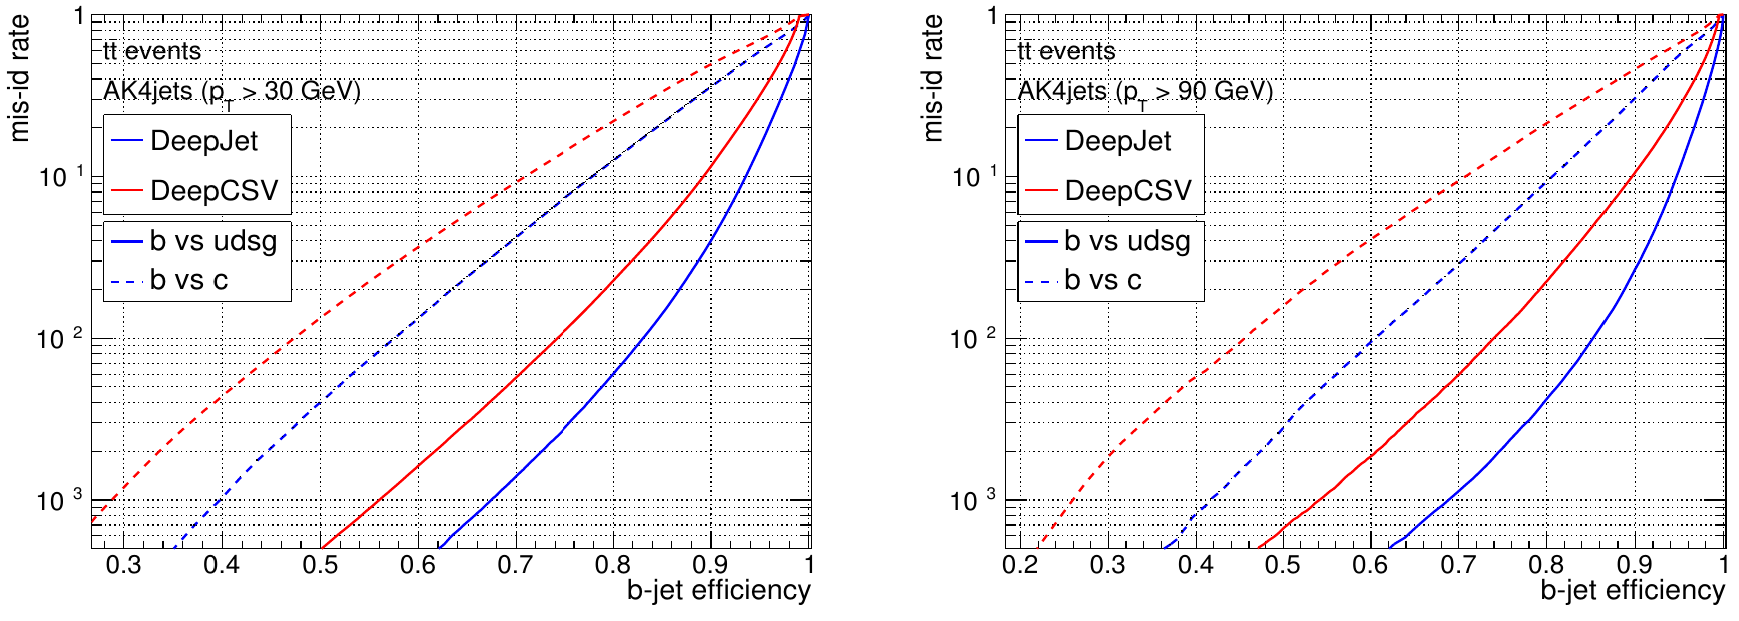
\includegraphics[width=\linewidth]{fig//chap04-reco/bjet.png}
    \caption{Performance comparison between \DeepJet and \DeepCSV, another model based on a simple feed-forward network. \cite{Bols2020JetDeepJet}}
    \label{fig:btag_perform}
\end{figure}



\section{Event simulation}
To optimize the analysis, estimate the efficiencies, evaluate the systematic uncertainties, and interpret the data, we need Monte Carlo simulations (MC): labeled data that reproduces the real data as faithfully as possible.\\
\\
The first stage of the simulation is the generation of the matrix elements, usually done with software like \MADGRAPH \cite{Alwall2011MadGraphBeyond} or \POWHEG \cite{Alioli2010ABOX}: after the user has defined all the Feynman diagrams to compute (including the initial and final state radiation) and the physics model, the four momenta of all the particles are computed at the parton level.
The next step, performed by \PYTHIA \cite{Sjostrand2006PYTHIAManual} in the CMS software, is the hadronization of colored particles, done exploiting the phenomenological Lund string model \cite{Andersson1983PartonDynamics}.\\
\\
The second step, performed by the \GEANTfour framework \cite{Agostinelli2003GEANT4--aToolkit}, is the simulation of the detector response and is the most computationally intensive step, to the point that other approaches to the simulation are being considered \cite{Sekmen2016RecentSimulation,Vaselli2023FlashSimFlow}.\\
\GEANT emulates the propagation of particles through the CMS detector, simulating the particle-matter interactions and the readout of each subdetector. In these steps, the electronic noise, the digitization, the Landau fluctuations, and all the inefficiencies of the detectors like the non-uniformity of the materials are simulated.\\
The events are then reconstructed exactly like the real data, with the same algorithms.\\
Despite the complexity of the full simulation, the MC can't reproduce exactly the real data so, for each analysis, the user has to apply the so-called scale factors (SF) to the MC, a set of event weights that represents the ratios of efficiencies between MC and data $SF=\epsilon_{data}/\epsilon_{MC}$.

